\documentclass[12pt, a4paper]{article}
\usepackage[utf8]{inputenc}

\title{Update of the register size used in the NeXtRad Synchronization Controller}
\author{Dominic Manthoko}
\date{\today}

%package needed in order to use images
\usepackage{graphicx}
\graphicspath{{images/}{images/tcu/}{images/tcu_external_clock}}

%hyperlinks
\usepackage{hyperref}
\hypersetup{
    colorlinks=true,
    linkcolor=blue,
    filecolor=magenta,      
    urlcolor=cyan,
}

\urlstyle{same}

%needed in order to make use of subfigures - figures stacked on top of one another or placed side by side
\usepackage{subcaption}

\setlength{\parindent}{0em}
\setlength{\parskip}{1em}

\begin{document}

%\begin{titlepage}
\maketitle
%\end{titlepage}

%Deals with the text being too long to fill one line
%E.g Background of the NeXtRad...
\sloppy


\section{Introduction}

\subsection{Subject and Motivation of Report}
The author was requested to make modifications to the NeXtRad Synchronization Controller developed by Johann Burger. In particular, the register size of the Synchronization Controller needed to be increased from 16 bits to 32 bits. 

\subsection{Background of the NeXtRad Synchronization Controller}


\subsection{Methodology}

\section{The Synchronization Controller}
\subsection{Modifications Made to the Original Synchronization Controller}
It is highly recommended that you read the document about the \href{https://docs.google.com/document/d/1E-mxDRlNcjSsjckUj8SuQOPBRs8Zv4AUUxXzLDHU3zc/edit?usp=sharing}{Timing Control Unit(TCU)}. This document specifies how to set up the synchronization controller, the commands used to operate it and so forth. In this section, only the parts that were modified will be mentioned.

\subsection{Setting up the Synchronization Controller} \label{syn_control_setup}
All the available registers can be accessed in the proc directory:

		\fbox{\begin{minipage}{30em}
		/proc/$<$PID$>$/hw/ioreg/
		\end{minipage}}

where $<$PID$>$ must be replaced by the process ID of the running firmware. This can be identified by running the ‘ps’ command in the terminal.

Registers can be written to by using the echo command. The following command writes a 1 to the n register:

	%display an example of the echo command inside a box
		\fbox{\begin{minipage}{30em}
			echo -e -n "\textbackslash x01\textbackslash x00" $>$ /proc/$<$PID$>$/hw/ioreg/n
		\end{minipage}}


The registers can then be read back by using the ‘od’ command:

	%display an example of the od command inside a box
	\fbox{\begin{minipage}{30em}
		od -x /proc/$<$PID$>$/hw/ioreg/n
	\end{minipage}}



%Explaining how to use the TCU with the modifications
With the modified TCU, reading and writing from the n, m and reg\textunderscore led registers found in the proc directory was left unchanged. The reg\textunderscore pulse register was altered such that it would be able to handle 32 bit values for the PRI offset.

%table describing the parameters used in the reg_pulses register
\begin{table}
\centering
\begin{tabular}{ |c|c|c|c| } 
 \hline
 Parameter & Size &  Description \\ 
 
 \hline 
 MB offset & 16 bits & Main Bang offset in 10ns intervals \\ 
 
 \hline
 DIG offset & 16 bits & Digitisation offset in 10ns intervals \\
 
 \hline
 Next PRI (upper 2 bytes) & 16 bits & Next PRI offset in 10ns intervals \\
 
 \hline
 Freq & 16 bits & Frequency of operation \\
 
 \hline
 Pol Mode & 3 btis & From table 1.2 \\
 
 \hline
 Next PRI (lower 2 bytes) & 16 bits & Next PRI offset in 10ns intervals\\
 \hline 
\end{tabular}
\caption{Table of all the parameters necessary for each pulse}
\label{table:1}
\end{table}

	\begin{figure}
		\centering
		\includegraphics[width=13cm]{reg_pulses}
		\caption{Visual depiction of how to order the parameters seen in Table \ref{table:1}}
		\label{fig:reg_pulses}
	\end{figure}



The original developer catered for the future improvement of the controller and had 16 bits of unused bits available for use. This free space was made use of in order to increase the register size of the PRI from 16- to 32-bits. In table \ref{table:1}, the various parameters required to set up a pulse are shown. Figure \ref{fig:reg_pulses} shows how the parameters seen in table \ref{table:1} would be setup using the echo command.


The parameters seen in table \ref{table:1} are set up by writing to the reg\textunderscore pulses register. If you wanted to set up a pulse that triggers every 1 ms (1Khz), has a main bang and digitisation offset of 500ns, a band frequency of 1300 MHz and operating at L-band, you would write the following command. 


	%display an example of the echo command inside a box
	\fbox{\begin{minipage}{30em}
			echo -e -n "\textbackslash x32\textbackslash x00\textbackslash x32\textbackslash x00\textbackslash x01\textbackslash x00\textbackslash x14\textbackslash x05\textbackslash x01\textbackslash x00\textbackslash x3b\textbackslash x86" $>$ /proc/$<$PID$>$/hw/ioreg/reg\textunderscore pulses
	\end{minipage}}


%how to get the hex values for the main bang offset and the digitization offset
The Rhino operates using a 100MHz clock, which is 10ns cycles. For the main bang and digitization offset, we divide the desired offset by 10ns to get the number of cycles. Since we want an offset of 500ns for both of them, the number of cycles is equal to 50 (x0032 in hexadecimal). The value must be in little endian thus we set these to \textbackslash x32\textbackslash x00. 


%how to get the hex values for the PRI offset
The desired PRI is calculated using the following equation:

	\[ 
		PRI = \frac{\frac{1}{PRF}}{10ns} - MB - D
	\]
Where
 
	\begin{itemize}
  		\item PRF is the frequency we want at the output i.e coming out of the main bang pin on the Rhino board
  		\item MB is the main bang offset in cycles
  		\item D is the digitization offset in cycles
	\end{itemize}

Since MB = D = 50 and we want a PRF of 1kHz, we get a value of 99899 for the PRI. Converting the value to hexadecimal we get x0001 863B. Then you would write \textbackslash x01\textbackslash x00 to PRI upper two bytes and \textbackslash x3b\textbackslash x86 to PRI lower two bytes.

\section{Experimental setup}

	\begin{figure}[h]
		\centering
		\includegraphics[width=13cm]{experimental_setup}
		\caption{Picture of the equipment used to test the 32 bit version of the synchronization controller}
		\label{fig:exp_setup}
	\end{figure}
	

The experimental setup used to test the modified controller can be seen in figure \ref{fig:exp_setup}. A signal generator operating at 100MHz with an amplitude of +550mV was used as the input clock. This clock signal was passed through a diode then fed into the rhino. An oscilloscope was used to measure the Main bang offset and Digitisation signals coming out of the rhino. 

A computer running the 64 bit version of xubuntu 16.04 LTS; which is a linux distribution based on ubuntu; was used to modify the VHDL code. Xilinx IDE verison 14.7 was used to edit the original TCU  project which can be found \href{https://github.com/Skippy01/NeXtRAD-TCU/tree/master/NeXtRAD-TCU-Controller}{here}.



\section{Results of the Experiment}

\subsection{Using the Rhino Board Internal 100MHz clock}

Testing of the modified synchronization controller began with using the internal clock of the Rhino board. Using the internal clock, 1kHz, 2kHz, 3kHz and 4kHz signals were produced. 

	\begin{figure}[h!]
		\centering
		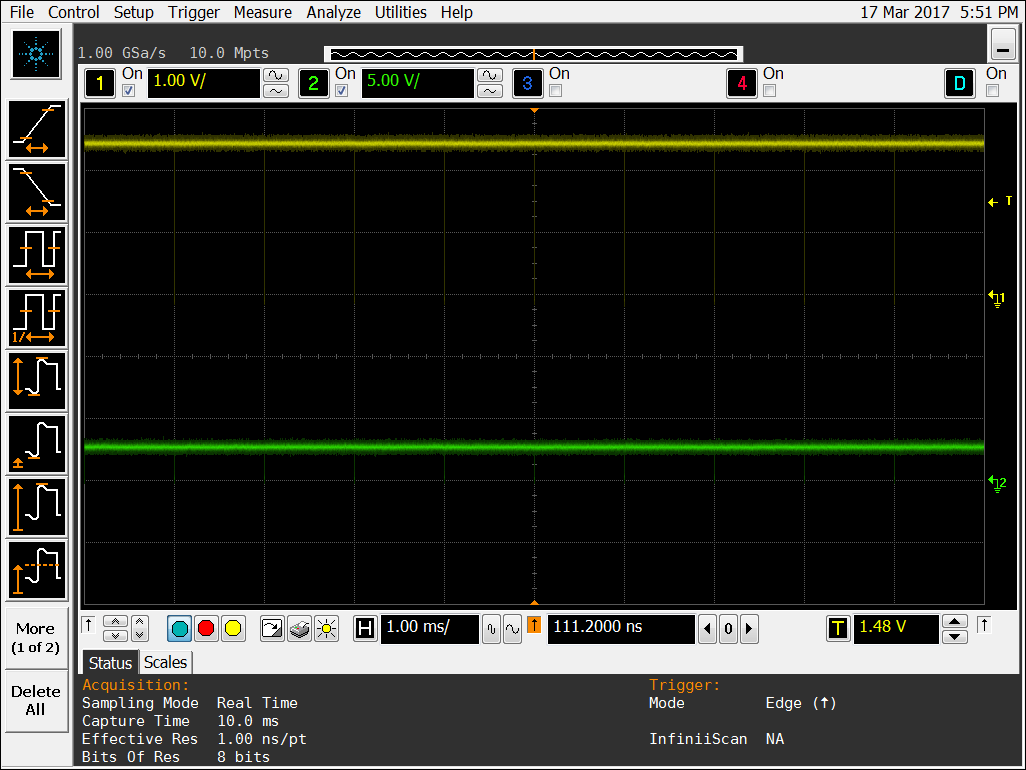
\includegraphics[width=13cm]{1khz_mb_offset_500_ns}
		\caption{1khz signal produced using the internal clock of the rhino}
		\label{fig:1khz_in_500_offset}
	\end{figure}
	
Figure \ref{fig:1khz_in_500_offset} shows the output of the main bang and the digitisation signals measured from the Rhino board. A time division of 1.0 ms was used to display the output. Observing the yellow signal, it can seen that a 1kHz signal is indeed being produced by the Rhino board.

	\begin{figure}[t]
		\centering
		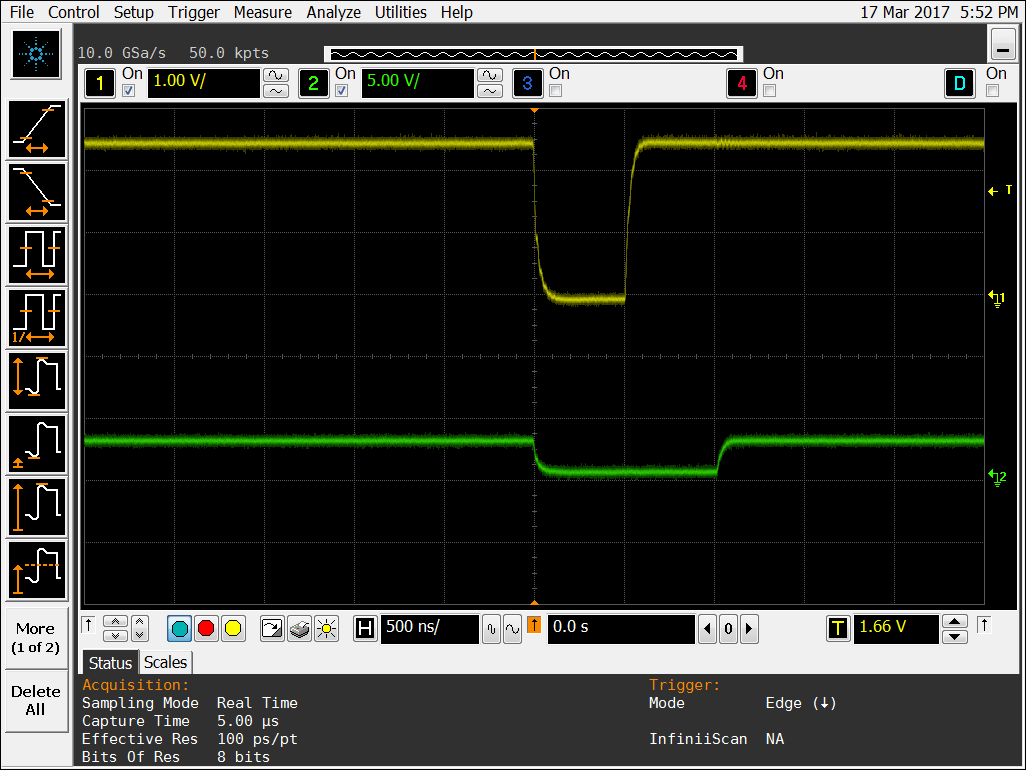
\includegraphics[width=13cm]{1khz_mb_offset_500_ns_length_of_offset}
		\caption{Zoomed in image of Figure \ref{fig:1khz_in_500_offset}}
		\label{fig:1khz_in_500_offset_zoom}
	\end{figure}
		
	
Figure \ref{fig:1khz_in_500_offset_zoom} shows a zoomed in image of Figure \ref{fig:1khz_in_500_offset}. The yellow signal depicts the main bang signal and the green signal depicts the digitization signal. The yellow signal goes high after 500ns and the green signal triggers 500ns after the yellow signal. These results are as desired. 

To change the main bang offset and the digitization offset to 1000ns without changing the other parameters, the following command was used:


	%display the echo command used to produce a signal with 1000ns offset
		\fbox{\begin{minipage}{30em}
			echo -e -n "\textbackslash x64\textbackslash x00\textbackslash x64\textbackslash x00\textbackslash x01\textbackslash x00\textbackslash x14\textbackslash x05\textbackslash x01\textbackslash x00\textbackslash x3b\textbackslash x86" $>$ /proc/$<$PID$>$/hw/ioreg/reg\textunderscore pulses
		\end{minipage}}
	
	%image showing that the main bang and digitization offset is indeed 1000ns
	\begin{figure}[t]
		\centering
		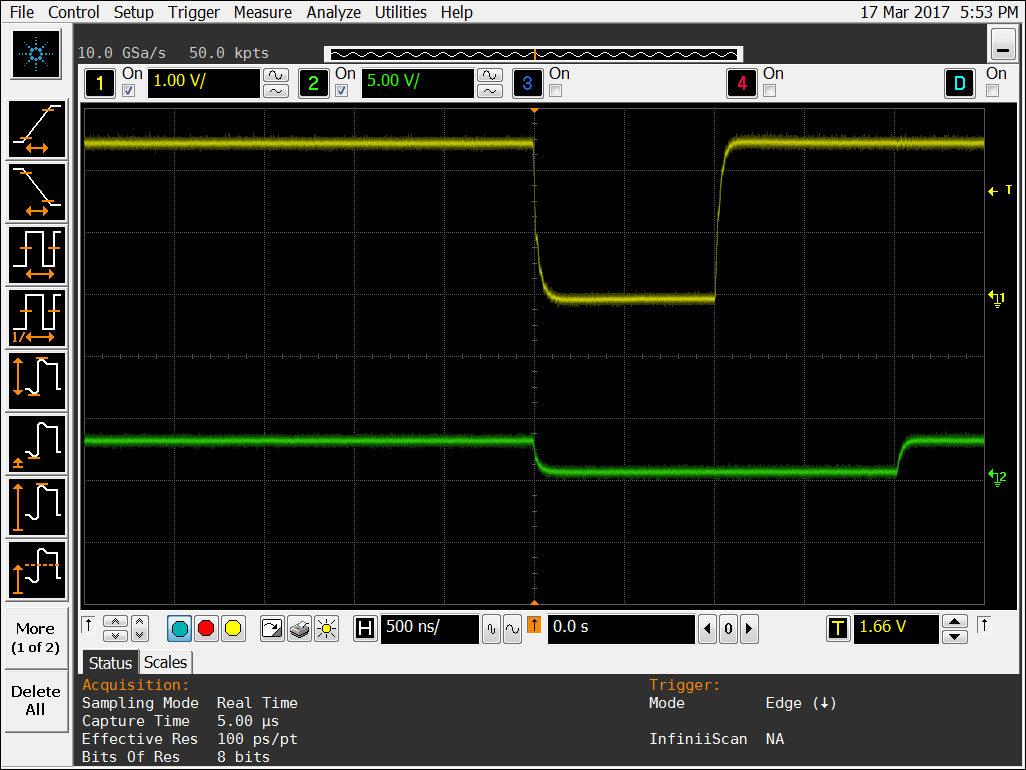
\includegraphics[width=13cm, height=8cm]{1khz_mb_offset_1000_ns_length_of_offset}
		\caption{Picture of the main bang signal and digitization with 1000ns offsets}
		\label{fig:1khz_in_1000_offset}
	\end{figure}
	

%explaining what is seen in the 1000ns image
Figure \ref{fig:1khz_in_1000_offset} shows a picture of the main bang and digitization signals with 1000ns offsets. Using the 500ns time division on the horizontal axis, it can be seen that it takes two time divisions for the main bang signal(yellow signal seen at the top of figure \ref{fig:1khz_in_1000_offset}) to go high. This equates to 1000ns, which is the desired result. Similarly for the digitization signal, we see that it also takes 2 time divisions to trigger, thus meeting our desired result. 

To show that the main bang offset and digitization offset can be set to different values, the main bang offset was set to 1650 ns and the digitization offset was set to 2950ns. The following command was used to set these values:

	%display the echo command used to produce a signal mb offset of 1650 ns 
	%and digitization offset of 2950ns
		\fbox{\begin{minipage}{30em}
			echo -e -n "\textbackslash xa5\textbackslash x00\textbackslash x27\textbackslash x01\textbackslash x01\textbackslash x00\textbackslash x14\textbackslash x05\textbackslash x01\textbackslash x00\textbackslash x3b\textbackslash x86" $>$ /proc/$<$PID$>$/hw/ioreg/reg\textunderscore pulses
		\end{minipage}}
		

	\begin{figure}[t]
		%\centering
   		\begin{subfigure}[t]{13.5cm}
   			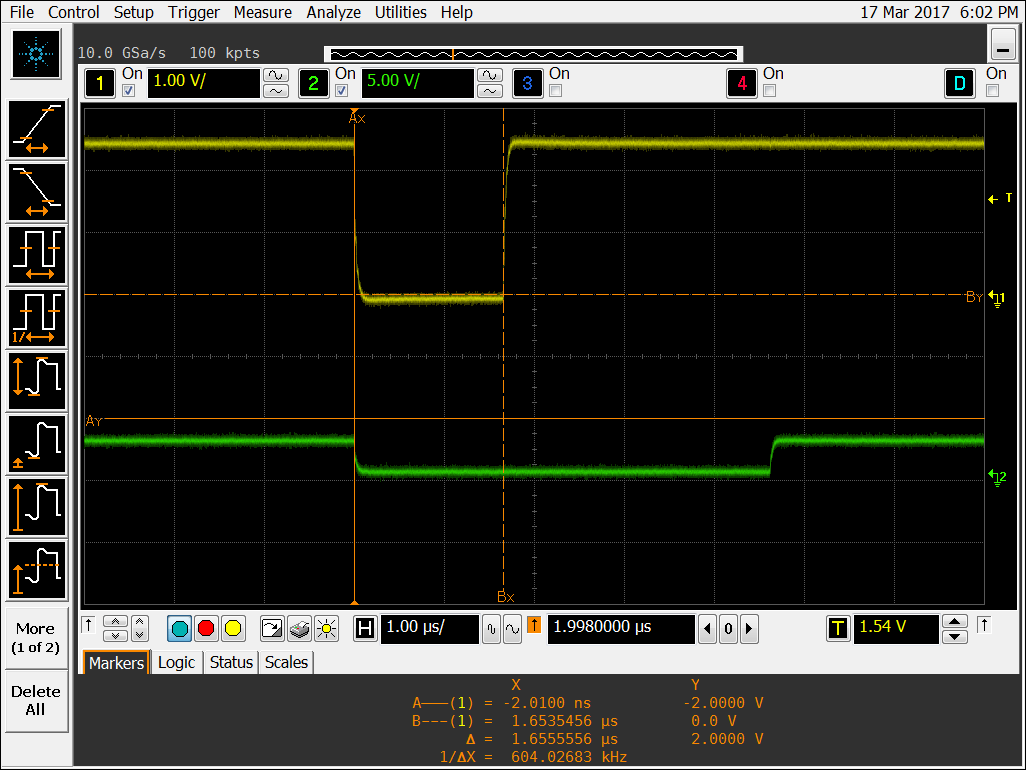
\includegraphics[width=13cm,height=8.5cm]{1khz_mb_1650ns_mb_offset}
   			\caption{}
   			\label{fig:var_offsets_1650} 
		\end{subfigure}

		\begin{subfigure}[t]{13.5cm}
   			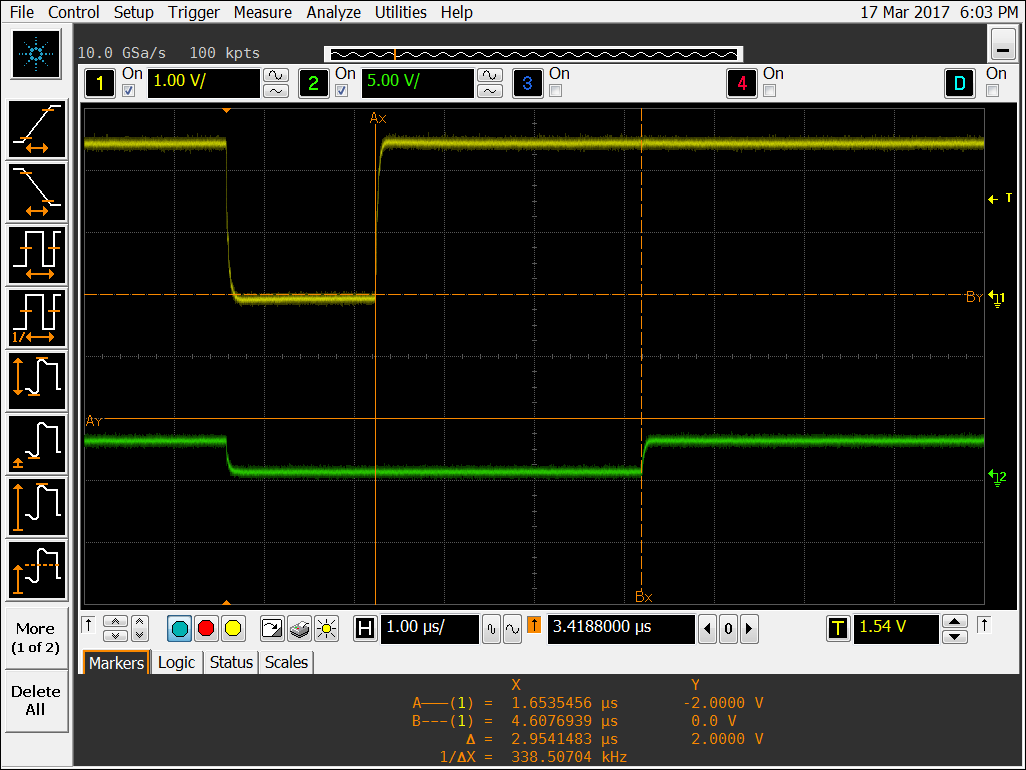
\includegraphics[width=13cm,height=8.5cm]{1khz_mb_2950ns_d_offset}
   			\caption{}
   		\label{fig:var_offsets_2950}
		\end{subfigure}

	\caption{(a) Main bang and digitization signal with the measurement of the main offset shown in the markers box toward the bottom of the image. (b) Same as figure \ref{fig:var_offsets_1650} but with the measurement of the digitization offset shown in the  markers box.}
	\label{fig:variable_offsets}
	\end{figure}
	
Figure \ref{fig:variable_offsets} shows the plots of the main bang signal and the digitization signal together with the measurements. Making use of cursors on the oscillscope, which allow you to measure a value on the horizontal and vertical axis, the offsets were measured. In the markers tab seen in figure \ref{fig:var_offsets_1650}, there is a delta value. From this plot, we see that \( \Delta = 1.6555556 \mu \). Observing the delta seen in figure \ref{fig:var_offsets_2950}, we see that \( \Delta = 2.9541483 \mu \). 


A main bang offset of 1650ns is equivalent to \( 1.65 \mu \). The value of delta seen in figure \ref{fig:var_offsets_1650} is thus approximately equal to the value that was set using the echo command. For the digitization offset, we set a value of 2950ns (\( 2.95 \mu \)). The delta value seen in figure \ref{fig:var_offsets_2950} is also approximately equal to the value that was set. This proves that the main bang and the digitization offsets can be set to two different values. 


	%image showing the 2khz signal using the internal clock
	%\begin{flushleft}
	\begin{figure}[t]
		\centering
		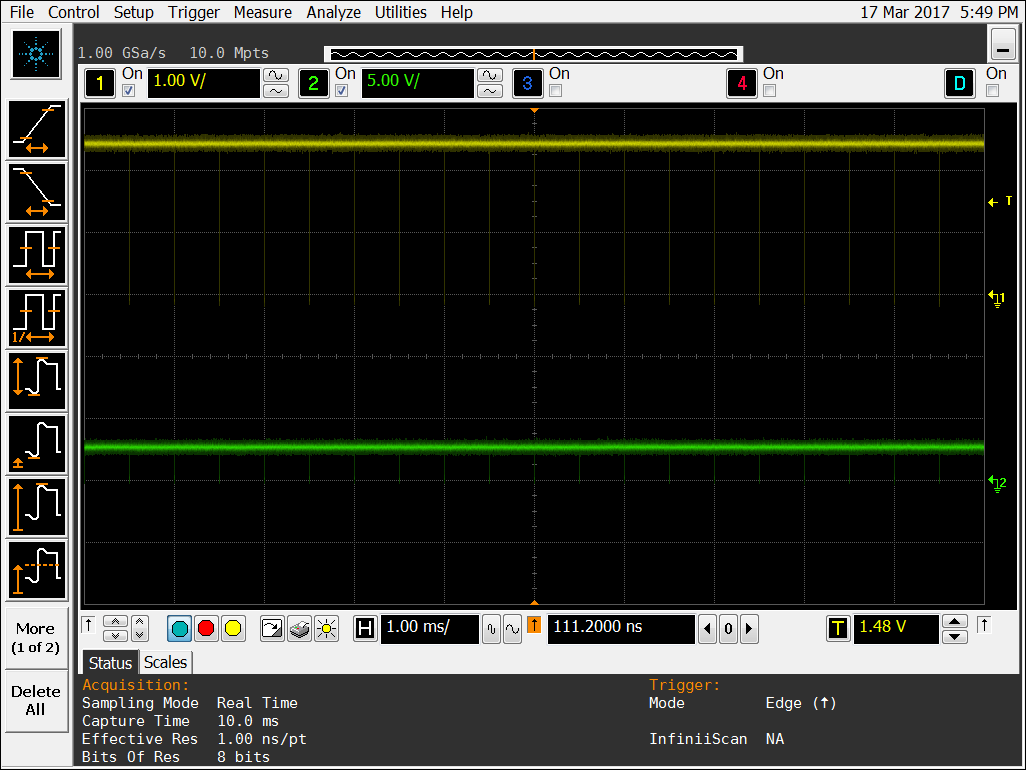
\includegraphics[width=13cm, height=8cm]{2khz_mb_offset_500_ns}
		\caption{Picture showing a 2khz signal produced using the internal clock of the Rhino board}
		\label{fig:2khz_sig_int}
	\end{figure}
	%\end{flushleft}	
	
	%image showing the 3khz signal using the internal clock
	%\begin{flushleft}
	\begin{figure}[t]
		\centering
		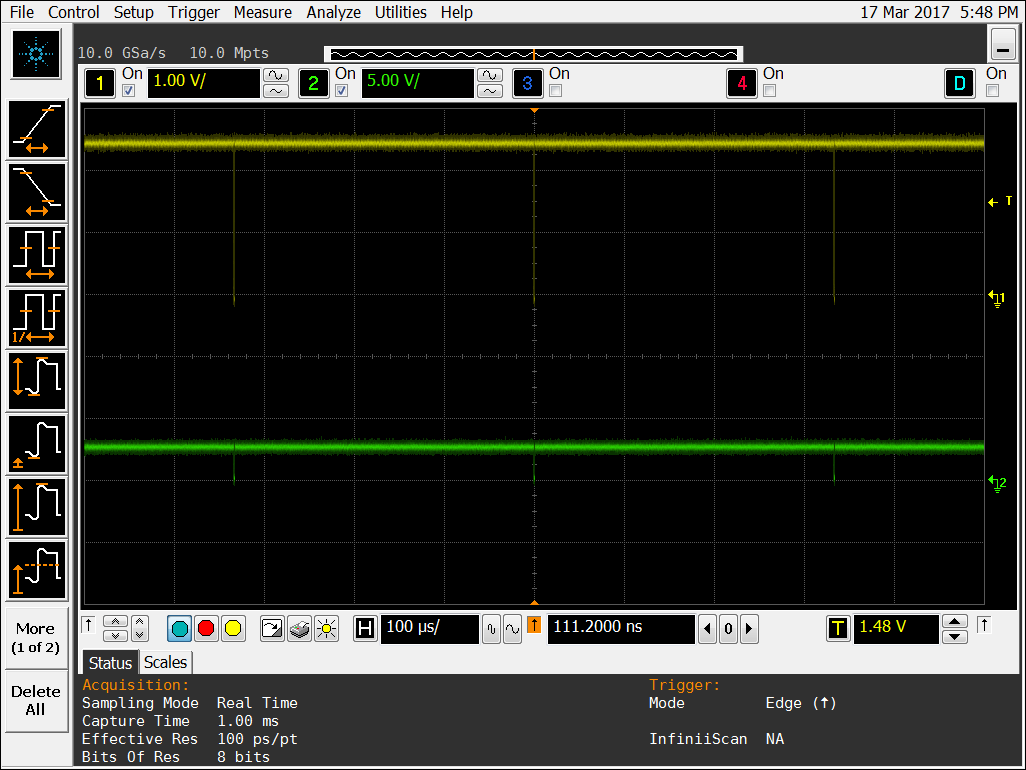
\includegraphics[width=13cm, height=8cm]{3khz_mb_offset_500_ns}
		\caption{Picture showing a 3khz signal produced using the internal clock of the Rhino board}
		\label{fig:3khz_sig_int}
	\end{figure}
	%\end{flushleft}
	
	%image showing the 4khz signal using the internal clock
	%\begin{flushleft}
	\begin{figure}[t]
		\centering
		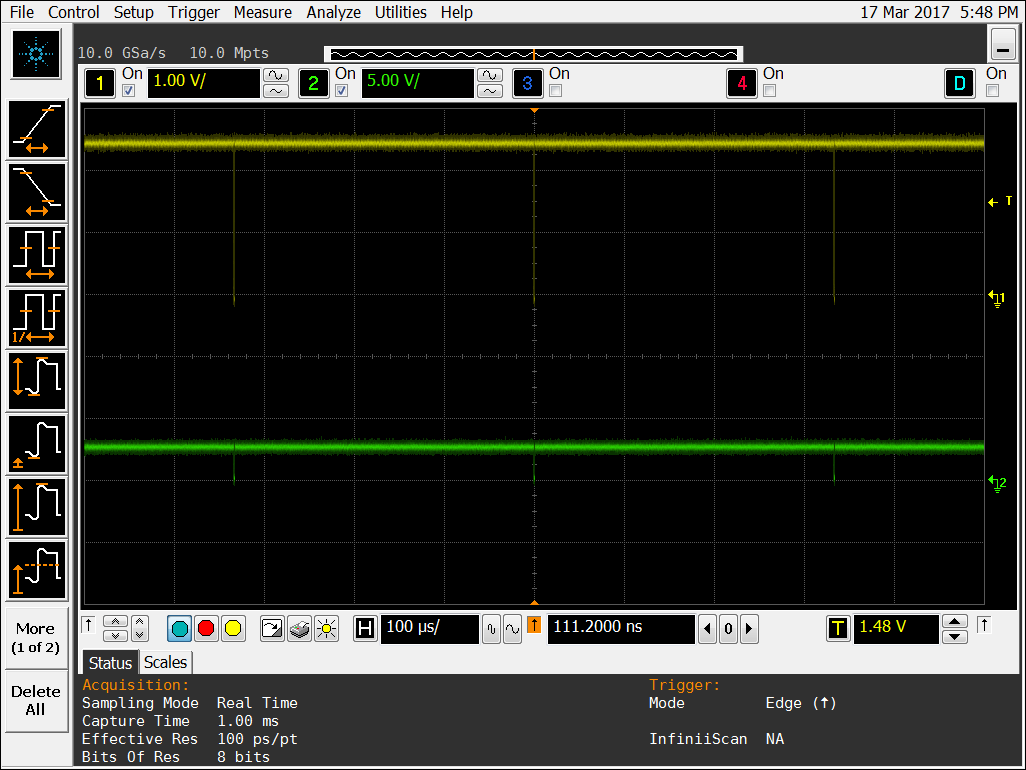
\includegraphics[width=13cm, height=8cm]{3khz_mb_offset_500_ns}
		\caption{Picture showing a 3khz signal produced using the internal clock of the Rhino board}
		\label{fig:4khz_sig_int}
	\end{figure}
	%\end{flushleft}		


Figures \ref{fig:2khz_sig_int}, \ref{fig:3khz_sig_int} and \ref{fig:4khz_sig_int} show pictures of the output produced when a signal with either a 2khz, 3khz or 4khz frequency is set using the echo command. Each of the plots was set using a 500ns offset for the main bang and digitization offsets, using a band frequency of 1300 Mhz, operating at L-band. The only that changes when switching between frequency is the PRI that is set. 


To produce a 2khz signal, we would need a PRI of 49899 (calculated using the equation for PRI found in section \ref{syn_control_setup}). The following command was used to set the parameters for the 2khz signal:
	
	%echo command used to set the 2khz signal
		\fbox{\begin{minipage}{30em}
			echo -e -n "\textbackslash x32\textbackslash x00\textbackslash x32\textbackslash x00\textbackslash x00\textbackslash x00\textbackslash x14\textbackslash x05\textbackslash x01\textbackslash x00\textbackslash xeb\textbackslash xc2" $>$ /proc/$<$PID$>$/hw/ioreg/reg\textunderscore pulses
		\end{minipage}}

\subsection{Using an External 100MHz Clock Signal}


\section{Conclusions}

\section{Recommendations}

\end{document}